% Created by tikzDevice version 0.6.1 on 2016-06-13 09:09:02
% !TEX encoding = UTF-8 Unicode
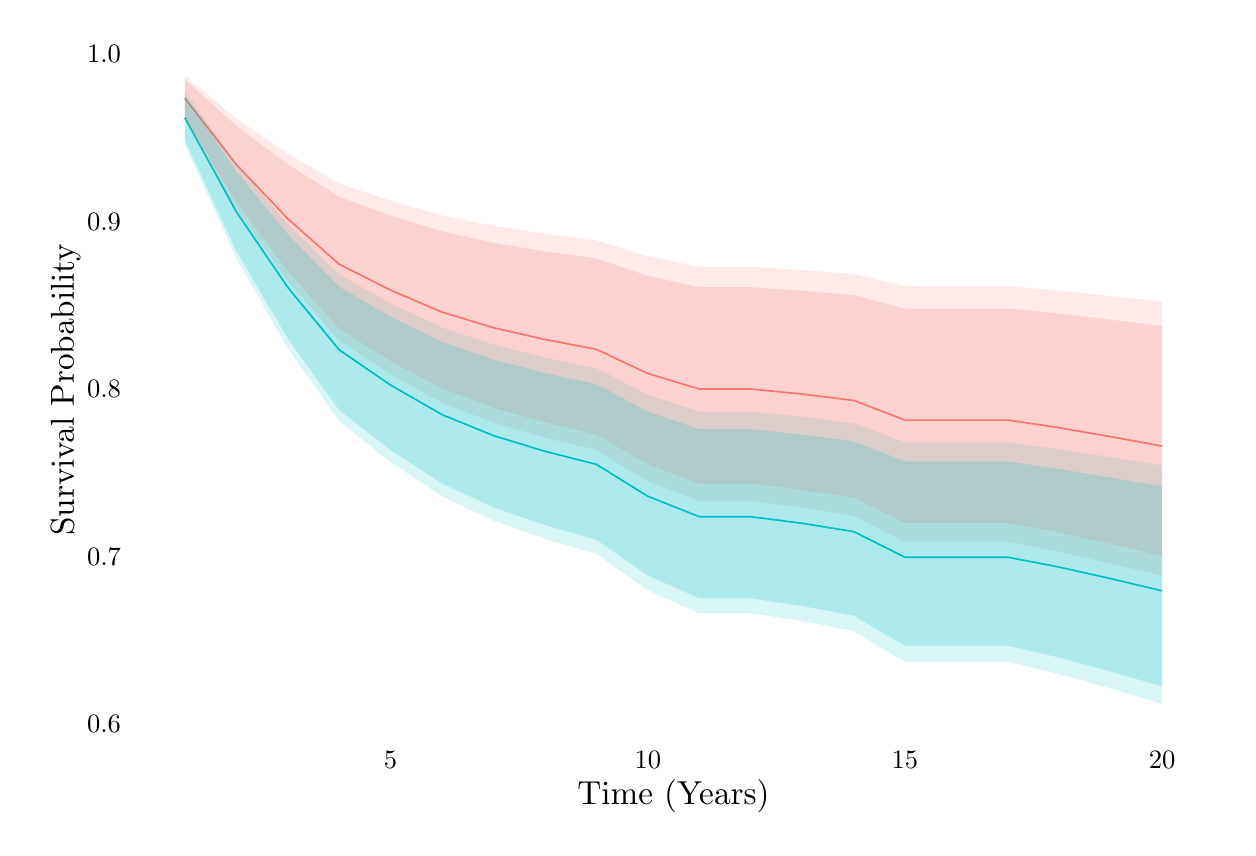
\begin{tikzpicture}[x=1pt,y=1pt]
\definecolor[named]{drawColor}{rgb}{0.00,0.00,0.00}
\definecolor[named]{fillColor}{rgb}{1.00,1.00,1.00}
\fill[color=fillColor,] (0,0) rectangle (433.62,289.08);
\begin{scope}
\path[clip] (  0.00,  0.00) rectangle (433.62,289.08);
\end{scope}
\begin{scope}
\path[clip] (  0.00,  0.00) rectangle (433.62,289.08);
\end{scope}
\begin{scope}
\path[clip] (  0.00,  0.00) rectangle (433.62,289.08);
\end{scope}
\begin{scope}
\path[clip] (  0.00,  0.00) rectangle (433.62,289.08);
\end{scope}
\begin{scope}
\path[clip] (  0.00,  0.00) rectangle (433.62,289.08);
\end{scope}
\begin{scope}
\path[clip] (  0.00,  0.00) rectangle (433.62,289.08);
\end{scope}
\begin{scope}
\path[clip] (  0.00,  0.00) rectangle (433.62,289.08);
\end{scope}
\begin{scope}
\path[clip] (  0.00,  0.00) rectangle (433.62,289.08);
\end{scope}
\begin{scope}
\path[clip] (  0.00,  0.00) rectangle (433.62,289.08);
\end{scope}
\begin{scope}
\path[clip] (  0.00,  0.00) rectangle (433.62,289.08);
\definecolor[named]{drawColor}{rgb}{1.00,1.00,1.00}
\definecolor[named]{fillColor}{rgb}{1.00,1.00,1.00}

\draw[color=drawColor,line width= 0.6pt,line cap=round,line join=round,fill=fillColor,] (  0.00,  0.00) rectangle (433.62,289.08);
\end{scope}
\begin{scope}
\path[clip] (  0.00,  0.00) rectangle (433.62,289.08);
\end{scope}
\begin{scope}
\path[clip] (  0.00,  0.00) rectangle (433.62,289.08);
\end{scope}
\begin{scope}
\path[clip] (  0.00,  0.00) rectangle (433.62,289.08);
\end{scope}
\begin{scope}
\path[clip] ( 39.13, 33.48) rectangle (427.62,283.08);
\definecolor[named]{fillColor}{rgb}{1.00,1.00,1.00}

\draw[fill=fillColor,draw opacity=0.00,] ( 39.13, 33.48) rectangle (427.62,283.08);
\definecolor[named]{drawColor}{rgb}{0.97,0.46,0.43}
\definecolor[named]{fillColor}{rgb}{0.97,0.46,0.43}

\draw[color=drawColor,line width= 0.6pt,line join=round,] ( 56.79,263.60) --
	( 75.38,239.65) --
	( 93.96,220.08) --
	(112.55,203.60) --
	(131.14,194.22) --
	(149.73,186.30) --
	(168.32,180.65) --
	(186.90,176.40) --
	(205.49,172.85) --
	(224.08,164.13) --
	(242.67,158.51) --
	(261.26,158.51) --
	(279.84,156.69) --
	(298.43,154.40) --
	(317.02,147.28) --
	(335.61,147.28) --
	(354.20,147.28) --
	(372.79,144.52) --
	(391.37,141.28) --
	(409.96,137.88);
\definecolor[named]{drawColor}{rgb}{0.00,0.75,0.77}
\definecolor[named]{fillColor}{rgb}{0.00,0.75,0.77}

\draw[color=drawColor,line width= 0.6pt,line join=round,] ( 56.79,256.55) --
	( 75.38,222.58) --
	( 93.96,195.30) --
	(112.55,172.67) --
	(131.14,159.93) --
	(149.73,149.25) --
	(168.32,141.68) --
	(186.90,136.01) --
	(205.49,131.28) --
	(224.08,119.76) --
	(242.67,112.37) --
	(261.26,112.37) --
	(279.84,109.99) --
	(298.43,106.99) --
	(317.02, 97.73) --
	(335.61, 97.73) --
	(354.20, 97.73) --
	(372.79, 94.15) --
	(391.37, 89.98) --
	(409.96, 85.60);
\definecolor[named]{fillColor}{rgb}{0.97,0.46,0.43}

\draw[fill=fillColor,fill opacity=0.15,draw opacity=0.00,] ( 56.79,271.73) --
	( 75.38,256.31) --
	( 93.96,243.62) --
	(112.55,232.71) --
	(131.14,226.52) --
	(149.73,221.24) --
	(168.32,217.44) --
	(186.90,214.56) --
	(205.49,212.18) --
	(224.08,206.43) --
	(242.67,202.67) --
	(261.26,202.67) --
	(279.84,201.48) --
	(298.43,200.04) --
	(317.02,195.70) --
	(335.61,195.70) --
	(354.20,195.70) --
	(372.79,194.06) --
	(391.37,192.09) --
	(409.96,190.04) --
	(409.96, 91.00) --
	(391.37, 95.47) --
	(372.79, 99.70) --
	(354.20,103.35) --
	(335.61,103.35) --
	(317.02,103.35) --
	(298.43,112.73) --
	(279.84,115.72) --
	(261.26,118.04) --
	(242.67,118.04) --
	(224.08,125.20) --
	(205.49,136.40) --
	(186.90,140.94) --
	(168.32,146.35) --
	(149.73,153.59) --
	(131.14,163.81) --
	(112.55,176.01) --
	( 93.96,197.52) --
	( 75.38,223.47) --
	( 56.79,255.59) --
	cycle;
\definecolor[named]{fillColor}{rgb}{0.00,0.75,0.77}

\draw[fill=fillColor,fill opacity=0.15,draw opacity=0.00,] ( 56.79,266.29) --
	( 75.38,239.97) --
	( 93.96,218.21) --
	(112.55,199.91) --
	(131.14,189.46) --
	(149.73,180.72) --
	(168.32,174.55) --
	(186.90,169.91) --
	(205.49,166.03) --
	(224.08,156.43) --
	(242.67,150.31) --
	(261.26,150.31) --
	(279.84,148.44) --
	(298.43,146.18) --
	(317.02,139.27) --
	(335.61,139.27) --
	(354.20,139.27) --
	(372.79,136.73) --
	(391.37,133.86) --
	(409.96,130.86) --
	(409.96, 44.82) --
	(391.37, 50.28) --
	(372.79, 55.50) --
	(354.20, 59.89) --
	(335.61, 59.89) --
	(317.02, 59.89) --
	(298.43, 71.06) --
	(279.84, 74.66) --
	(261.26, 77.45) --
	(242.67, 77.45) --
	(224.08, 85.87) --
	(205.49, 98.99) --
	(186.90,104.42) --
	(168.32,110.96) --
	(149.73,119.74) --
	(131.14,132.09) --
	(112.55,146.85) --
	( 93.96,173.36) --
	( 75.38,205.73) --
	( 56.79,246.96) --
	cycle;
\definecolor[named]{fillColor}{rgb}{0.97,0.46,0.43}

\draw[fill=fillColor,fill opacity=0.20,draw opacity=0.00,] ( 56.79,270.42) --
	( 75.38,253.60) --
	( 93.96,239.77) --
	(112.55,227.93) --
	(131.14,221.20) --
	(149.73,215.47) --
	(168.32,211.35) --
	(186.90,208.24) --
	(205.49,205.65) --
	(224.08,199.39) --
	(242.67,195.31) --
	(261.26,195.31) --
	(279.84,194.01) --
	(298.43,192.42) --
	(317.02,187.59) --
	(335.61,187.59) --
	(354.20,187.59) --
	(372.79,185.76) --
	(391.37,183.56) --
	(409.96,181.27) --
	(409.96, 98.21) --
	(391.37,102.52) --
	(372.79,106.61) --
	(354.20,110.13) --
	(335.61,110.13) --
	(317.02,110.13) --
	(298.43,119.17) --
	(279.84,122.06) --
	(261.26,124.31) --
	(242.67,124.31) --
	(224.08,131.25) --
	(205.49,142.07) --
	(186.90,146.47) --
	(168.32,151.70) --
	(149.73,158.71) --
	(131.14,168.58) --
	(112.55,180.35) --
	( 93.96,201.08) --
	( 75.38,226.04) --
	( 56.79,256.87) --
	cycle;
\definecolor[named]{fillColor}{rgb}{0.00,0.75,0.77}

\draw[fill=fillColor,fill opacity=0.20,draw opacity=0.00,] ( 56.79,264.72) --
	( 75.38,237.14) --
	( 93.96,214.46) --
	(112.55,195.43) --
	(131.14,184.60) --
	(149.73,175.52) --
	(168.32,169.11) --
	(186.90,164.29) --
	(205.49,160.27) --
	(224.08,150.34) --
	(242.67,143.99) --
	(261.26,143.99) --
	(279.84,142.04) --
	(298.43,139.65) --
	(317.02,132.33) --
	(335.61,132.33) --
	(354.20,132.33) --
	(372.79,129.61) --
	(391.37,126.51) --
	(409.96,123.26) --
	(409.96, 51.09) --
	(391.37, 56.40) --
	(372.79, 61.46) --
	(354.20, 65.74) --
	(335.61, 65.74) --
	(317.02, 65.74) --
	(298.43, 76.63) --
	(279.84, 80.14) --
	(261.26, 82.87) --
	(242.67, 82.87) --
	(224.08, 91.14) --
	(205.49,104.03) --
	(186.90,109.35) --
	(168.32,115.76) --
	(149.73,124.36) --
	(131.14,136.46) --
	(112.55,150.91) --
	( 93.96,176.83) --
	( 75.38,208.40) --
	( 56.79,248.49) --
	cycle;
\end{scope}
\begin{scope}
\path[clip] (  0.00,  0.00) rectangle (433.62,289.08);
\end{scope}
\begin{scope}
\path[clip] (  0.00,  0.00) rectangle (433.62,289.08);
\end{scope}
\begin{scope}
\path[clip] (  0.00,  0.00) rectangle (433.62,289.08);
\end{scope}
\begin{scope}
\path[clip] (  0.00,  0.00) rectangle (433.62,289.08);
\end{scope}
\begin{scope}
\path[clip] (  0.00,  0.00) rectangle (433.62,289.08);
\end{scope}
\begin{scope}
\path[clip] (  0.00,  0.00) rectangle (433.62,289.08);
\definecolor[named]{drawColor}{rgb}{0.00,0.00,0.00}

\node[color=drawColor,anchor=base east,inner sep=0pt, outer sep=0pt, scale=  0.96] at ( 33.73, 34.25) {0.6%
};

\node[color=drawColor,anchor=base east,inner sep=0pt, outer sep=0pt, scale=  0.96] at ( 33.73, 94.77) {0.7%
};

\node[color=drawColor,anchor=base east,inner sep=0pt, outer sep=0pt, scale=  0.96] at ( 33.73,155.30) {0.8%
};

\node[color=drawColor,anchor=base east,inner sep=0pt, outer sep=0pt, scale=  0.96] at ( 33.73,215.82) {0.9%
};

\node[color=drawColor,anchor=base east,inner sep=0pt, outer sep=0pt, scale=  0.96] at ( 33.73,276.35) {1.0%
};
\end{scope}
\begin{scope}
\path[clip] (  0.00,  0.00) rectangle (433.62,289.08);
\end{scope}
\begin{scope}
\path[clip] (  0.00,  0.00) rectangle (433.62,289.08);
\end{scope}
\begin{scope}
\path[clip] (  0.00,  0.00) rectangle (433.62,289.08);
\end{scope}
\begin{scope}
\path[clip] (  0.00,  0.00) rectangle (433.62,289.08);
\end{scope}
\begin{scope}
\path[clip] (  0.00,  0.00) rectangle (433.62,289.08);
\end{scope}
\begin{scope}
\path[clip] (  0.00,  0.00) rectangle (433.62,289.08);
\end{scope}
\begin{scope}
\path[clip] (  0.00,  0.00) rectangle (433.62,289.08);
\end{scope}
\begin{scope}
\path[clip] (  0.00,  0.00) rectangle (433.62,289.08);
\end{scope}
\begin{scope}
\path[clip] (  0.00,  0.00) rectangle (433.62,289.08);
\end{scope}
\begin{scope}
\path[clip] (  0.00,  0.00) rectangle (433.62,289.08);
\end{scope}
\begin{scope}
\path[clip] (  0.00,  0.00) rectangle (433.62,289.08);
\end{scope}
\begin{scope}
\path[clip] (  0.00,  0.00) rectangle (433.62,289.08);
\definecolor[named]{drawColor}{rgb}{0.00,0.00,0.00}

\node[color=drawColor,anchor=base,inner sep=0pt, outer sep=0pt, scale=  0.96] at (131.14, 21.46) {5%
};

\node[color=drawColor,anchor=base,inner sep=0pt, outer sep=0pt, scale=  0.96] at (224.08, 21.46) {10%
};

\node[color=drawColor,anchor=base,inner sep=0pt, outer sep=0pt, scale=  0.96] at (317.02, 21.46) {15%
};

\node[color=drawColor,anchor=base,inner sep=0pt, outer sep=0pt, scale=  0.96] at (409.96, 21.46) {20%
};
\end{scope}
\begin{scope}
\path[clip] (  0.00,  0.00) rectangle (433.62,289.08);
\end{scope}
\begin{scope}
\path[clip] (  0.00,  0.00) rectangle (433.62,289.08);
\end{scope}
\begin{scope}
\path[clip] (  0.00,  0.00) rectangle (433.62,289.08);
\end{scope}
\begin{scope}
\path[clip] (  0.00,  0.00) rectangle (433.62,289.08);
\definecolor[named]{drawColor}{rgb}{0.00,0.00,0.00}

\node[color=drawColor,anchor=base,inner sep=0pt, outer sep=0pt, scale=  1.20] at (233.37,  8.40) {Time (Years)%
};
\end{scope}
\begin{scope}
\path[clip] (  0.00,  0.00) rectangle (433.62,289.08);
\end{scope}
\begin{scope}
\path[clip] (  0.00,  0.00) rectangle (433.62,289.08);
\definecolor[named]{drawColor}{rgb}{0.00,0.00,0.00}

\node[rotate= 90.00,color=drawColor,anchor=base,inner sep=0pt, outer sep=0pt, scale=  1.20] at ( 16.66,158.28) {Survival Probability%
};
\end{scope}
\begin{scope}
\path[clip] (  0.00,  0.00) rectangle (433.62,289.08);
\end{scope}
\begin{scope}
\path[clip] (  0.00,  0.00) rectangle (433.62,289.08);
\end{scope}
\begin{scope}
\path[clip] (  0.00,  0.00) rectangle (433.62,289.08);
\end{scope}
\begin{scope}
\path[clip] (  0.00,  0.00) rectangle (433.62,289.08);
\end{scope}
\end{tikzpicture}
